%!TEX root = /Users/ego/Boulot/TKZ/tkz-euclide/doc_fr/TKZdoc-euclide-main.tex

\section{Les segments}

Il existe bien sûr, une macro pour tracer simplement un segment (il serait possible comme pour une demi-droite, de créer un style avec \tkzcname{add}) .

\subsection{Tracer un segment \tkzcname{tkzDrawSegment}} 
 \hypertarget{tds}{}      

 \begin{NewMacroBox}{tkzDrawSegment}{\oarg{local options}\parg{pt1,pt2}}
\emph{Les arguments sont une liste de deux points. Les styles de \TIKZ\ sont accessibles pour les tracés}
 
\medskip
\begin{tabular}{lll}
argument    & exemple & définition    \\
\midrule
\TAline{(pt1,pt2)}{(A,B)}{trace le segment $[A,B]$}
\bottomrule 
\end{tabular}

C'est bien sûr équivalent à \tkzcname{draw (A)--(B);} 
\end{NewMacroBox}

\subsubsection{Exemple avec des références de points}     

\begin{tkzexample}[latex=6cm]
\begin{tikzpicture}[scale=1.5]
  \tkzInit[xmin=-1,xmax=3,ymin=-1,ymax=2]
  \tkzClip
  \tkzDefPoint(0,0){A}
  \tkzDefPoint(2,1){B}
  \tkzDrawSegment[color=red,thin](A,B)
  \tkzDrawPoints(A,B)    
  \tkzLabelPoints(A,B)  
\end{tikzpicture}
\end{tkzexample}
  

\subsubsection{Exemple avec des références de points} 
 Il est préférable de référencer les points, car les points sont
 placées en tenant compte de  \tkzcname{tkzInit}.
 
\begin{tkzexample}[latex=6cm]
\begin{tikzpicture}[scale=1.5]
  \tkzInit[xmin=-1,xmax=3,ymin=-1,ymax=2]
  \tkzClip
  \tkzDrawSegment[color=red,thin]({0,0},{2,1})  
\end{tikzpicture}
\end{tkzexample} 

\bigskip
Si les options sont les mêmes on peut tracer plusieurs \hypertarget{segs}{segments} avec la même macro. 
 
\newpage
\subsection{Tracer des segments \tkzcname{tkzDrawSegments}} 
 \hypertarget{tdss}{}      

 \begin{NewMacroBox}{tkzDrawSegments}{\oarg{local options}\parg{pt1,pt2 pt3,pt4 ...}}
\emph{Les arguments sont une liste de couple de deux points. Les styles de \TIKZ\ sont accessibles pour les tracés}
\end{NewMacroBox}

\begin{center}
\begin{tkzexample}[latex=6cm]
\begin{tikzpicture}
  \tkzInit[xmin=-1,xmax=3,ymin=-1,ymax=2]
  \tkzClip[space=1]
  \tkzDefPoint(0,0){A}
  \tkzDefPoint(2,1){B} 
  \tkzDefPoint(3,0){C} 
  \tkzDrawSegments(A,B B,C)
  \tkzDrawPoints(A,B,C)    
  \tkzLabelPoints(A,C) 
  \tkzLabelPoints[above](B)  
\end{tikzpicture}
\end{tkzexample}
\end{center} 

\subsection{Marquer un segment \tkzcname{tkzMarkSegment}}
\hypertarget{tms}{}  
  
 \begin{NewMacroBox}{tkzMarkSegment}{\oarg{local options}\parg{pt1,pt2}} 
\emph{La macro permet de placer une marque sur un segment.}

\medskip
\begin{tabular}{lll}
\toprule
options             & défaut & définition    \\
\midrule
\TOline{pos}{.5}{position de la marque} 
\TOline{color}{black}{couleur de la marque} 
\TOline{mark}{none}{choix de la marque} 
\TOline{size}{4pt}{taille de la marque} 
\bottomrule
\end{tabular}

\emph{Les marques possibles sont celles fournies par \TIKZ, mais d'autres marques ont été crées d'après une idée de Yves Combe.}
\end{NewMacroBox} 

\subsubsection{Marques multiples}
\begin{tkzexample}[latex=6cm,small] 
\begin{tikzpicture}
  \tkzDefPoint(2,1){A}
  \tkzDefPoint(6,4){B}
  \tkzDrawSegment(A,B)
  \tkzMarkSegment[color=Maroon,size=2pt,
        pos=0.4, mark=z](A,B) 
  \tkzMarkSegment[color=blue,
        pos=0.2, mark=oo](A,B)
  \tkzMarkSegment[pos=0.8,
        mark=s,color=red](A,B) 
\end{tikzpicture}
\end{tkzexample}

\subsubsection{Utilisation de \tkzname{mark}}      
\begin{tkzexample}[latex=6cm,small] 
\begin{tikzpicture}
  \tkzDefPoint(2,1){A} 
  \tkzDefPoint(6,4){B}
  \tkzDrawSegment(A,B)
  \tkzMarkSegment[color=gray,
                  pos=0.2,mark=s|](A,B)
  \tkzMarkSegment[color=gray,
                  pos=0.4,mark=s||](A,B)
  \tkzMarkSegment[color=Maroon,
                  pos=0.6,mark=||](A,B)
  \tkzMarkSegment[color=red,
                  pos=0.8,mark=|||](A,B)
\end{tikzpicture}
\end{tkzexample}


\subsection{Marquer des segments \tkzcname{tkzMarkSegments}}
\hypertarget{tmss}{} 
 
\begin{NewMacroBox}{tkzMarkSegments}{\oarg{local options}\parg{pt1,pt2 pt3,pt4 ...}}
\emph{Les arguments sont une liste de couple de deux points séparés par des espaces. Les styles de \TIKZ\ sont accessibles pour les tracés.}
\end{NewMacroBox} 

\subsubsection{Marques pour un triangle isocèle}      
\begin{tkzexample}[latex=6cm,small]
\begin{tikzpicture}[scale=1]
 \tkzDefPoints{0/0/O,2/2/A,4/0/B,6/2/C}
 \tkzDrawSegments(O,A A,B)
 \tkzDrawPoints(O,A,B)
 \tkzDrawLine(O,B)   
 \tkzMarkSegments[mark=||,size=6pt](O,A A,B)
\end{tikzpicture}
\end{tkzexample} 

\subsection{Exemple de rotation}   
\begin{center}
\begin{tkzexample}[latex=7cm,small] 
 \begin{tikzpicture}[scale=0.5]
  \tkzDefPoint(0,0){A}\tkzDefPoint(3,2){B} 
  \tkzDefPoint(4,0){C}\tkzDefPoint(2.5,1){P}
  \tkzDrawPolygon(A,B,C)
  \tkzDefEquilateral(A,P) \tkzGetPoint{P'}
  \tkzDefPointsBy[rotation=center A angle 60](P,B){P',C'}
  \tkzDrawPolygon(A,P,P')
  \tkzDrawPolySeg(P',C',A,P,B)
  \tkzDrawSegment(C,P)
  \tkzDrawPoints(A,B,C,C',P,P')
  \tkzMarkSegments[mark=s|,mark size=6pt,
  color=blue](A,P P,P' P',A) 
  \tkzMarkSegments[mark=||,color=orange](B,P P',C')
  \tkzLabelPoints(A,C) \tkzLabelPoints[below](P) 
  \tkzLabelPoints[above right](P',C',B) 
  
\end{tikzpicture} 
\end{tkzexample}  
\end{center}  
\newpage  
\hypertarget{tls}{}  
 \begin{NewMacroBox}{tkzLabelSegment}{\oarg{local options}\parg{pt1,pt2}\marg{label}}
\emph{Cette macro permet de placer une étiquette le long d'un segment ou encore d'une ligne. Les options sont celles de \TIKZ\ par exemple \tkzname{pos} } 

\medskip
\begin{tabular}{lll}
argument    & exemple & définition    \\
\midrule
\TAline{label}{\tkzcname{tkzLabelSegment(A,B)\{$5$\}}}{texte de l'étiquette} 
\TAline{(pt1,pt2)}{(A,B)}{étiquette le long de $[A,B]$} 
\bottomrule
\end{tabular}


\medskip
\begin{tabular}{lll}
options  & défaut & définition    \\
\midrule
\TOline{pos}{.5}{position du label} 
\end{tabular}
\end{NewMacroBox}  

 \subsubsection{Labels multiples}      
\begin{tkzexample}[latex=6 cm,small]
\begin{tikzpicture}
\tkzInit
\tkzDefPoint(0,0){A}
\tkzDefPoint(6,0){B}
\tkzDrawSegment(A,B)
\tkzLabelSegment[above,pos=.8](A,B){$a$}
\tkzLabelSegment[below,pos=.2](A,B){$4$}
\end{tikzpicture} 
\end{tkzexample}  

\subsubsection{Labels et Pythagore}
Cet exemple nécessite \tkzcname{usetkzobj{polygons}}
      
\begin{tkzexample}[latex=7cm]
\begin{tikzpicture}[scale=.75]
\tkzInit[xmax=5,ymax=5]
\tkzDefPoint(0,0){C}
\tkzDefPoint(4,0){A}
\tkzDefPoint(0,3){B}
\tkzDefSquare(B,A)\tkzGetPoints{E}{F}
\tkzDefSquare(A,C)\tkzGetPoints{G}{H}
\tkzDefSquare(C,B)\tkzGetPoints{I}{J}
\tkzFillPolygon[draw,
                fill = red!50 ](A,C,G,H)
\tkzFillPolygon[draw,
                fill = blue!50 ](C,B,I,J)
\tkzFillPolygon[draw,
                fill = purple!50](B,A,E,F)
\tkzFillPolygon[draw,opacity=.5,
                fill = orange](A,B,C)
\tkzDrawPolygon[line width = 1pt](A,B,C)
\tkzLabelSegment[above](C,A){$a$}
\tkzLabelSegment[right](B,C){$b$}
\tkzLabelSegment[below left](B,A){$c$}
\end{tikzpicture} 
\end{tkzexample}

\newpage 
\hypertarget{tlss}{} 
 \begin{NewMacroBox}{tkzLabelSegments}{\oarg{local options}\parg{pt1,pt2 pt3,pt4 ...}}
\emph{Les arguments sont une liste de couple de deux points. Les styles de \TIKZ\ sont accessibles pour les tracés.}
\end{NewMacroBox} 
 
\subsubsection{Labels pour un triangle isocèle}      
\begin{center}
\begin{tkzexample}[latex=6cm,small]
\begin{tikzpicture}[scale=1]
 \tkzDefPoints{0/0/O,2/2/A,4/0/B,6/2/C}
 \tkzDrawSegments(O,A A,B)
 \tkzDrawPoints(O,A,B)
 \tkzDrawLine(O,B)   
 \tkzLabelSegments[color=red,above=4pt](O,A A,B){$a$}
\end{tikzpicture}
\end{tkzexample}  
\end{center}   
\endinput


